%%%%%%%%%%%%%%%%%%%%%%%%%%%%%% -*- Mode: Latex -*- %%%%%%%%%%%%%%%%%%%%%%%%%%%%
%% project.tex -- 
%% Author          : Philip Johnson
%% Created On      : Tue Mar 31 11:44:58 2009
%% Last Modified By: Philip Johnson
%% Last Modified On: Thu Jan 26 11:19:10 2012
%%%%%%%%%%%%%%%%%%%%%%%%%%%%%%%%%%%%%%%%%%%%%%%%%%%%%%%%%%%%%%%%%%%%%%%%%%%%%%%

\documentclass{proposalnsf}
\usepackage[final]{graphicx}
\usepackage{url}

% NSF proposal generation template style file.
% based on latex stylefiles  written by Stefan Llewellyn Smith and
% Sarah Gille, with contributions from other collaborators.

\renewcommand{\refname}{\centerline{References cited}}

% Fix things so that figures tend to stay away from the last page. 
\renewcommand{\topfraction}{0.85}
\renewcommand{\textfraction}{0.1}
\renewcommand{\floatpagefraction}{0.75}

% this handles hanging indents for publications
\def\rrr#1\\{\par
\medskip\hbox{\vbox{\parindent=2em\hsize=6.12in
\hangindent=4em\hangafter=1#1}}}

\def\baselinestretch{1}

\renewcommand{\thefootnote}{}

\begin{document}



% \pagenumbering{arabic}
% \renewcommand{\thepage} {C--\arabic{page}}
% \renewcommand{\thesection} {C.\arabic{section}}
% \setcounter{section}{0}

\section{Project Description}

\tableofcontents

%%%%%%%%%%%%%%%%%%%%%%%%%%%%%% -*- Mode: Latex -*- %%%%%%%%%%%%%%%%%%%%%%%%%%%%
%% project.intro.tex -- 
%% Author          : Philip Johnson
%% Created On      : Fri Jan 13 19:47:12 2012
%% Last Modified By: Philip Johnson
%% Last Modified On: Wed Jan 18 13:13:30 2012
%%%%%%%%%%%%%%%%%%%%%%%%%%%%%%%%%%%%%%%%%%%%%%%%%%%%%%%%%%%%%%%%%%%%%%%%%%%%%%%

\subsection{Introduction}

Development of the ``Smart Grid'', a modernized power infrastructure, is
one of the key technological challenges facing the United States at the
dawn of the 21st century. According to the Department of Energy (DoE) , the smart
grid should: (1) Enable active participation by consumers by providing
choices and incentives to modify electricity purchasing patterns and
behavior; (2) Accommodate all generation and storage options, including
wind and solar power.  (3) Enable new products, services, and markets
through a flexible market providing cost-benefit trade-offs to consumers
and market participants; (4) Provide reliable power that is relatively
interruption-free; (5) Optimize asset utilization and maximize operational
efficiency; (6) Provide the ability to self-heal by anticipating and
responding to system disturbances; (7) Resist attacks on physical
infrastructure by natural disasters and attacks on cyber-structure by
malware and hackers \cite{NETL:GridCharacteristics}.

Supporting ``all generation options'' implies the need to support
distributed, small scale, intermittent generation such as residential
solar.  Supporting ``all storage options'' implies the need to support
distributed, small scale, intermittent storage such as electric vehicle
batteries.  Once energy generation and storage can be just as decentralized
as energy consumption, the utility of microgrids as a building block for
the DoE Smart Grid becomes clear.  Microgrids are semi-autonomous,
self-regulating electrical systems below the subsystem level that can
involve small-scale storage and generation as well as consumption.

\subsubsection{Vision}
\label{sec:vision}

\footnote{Section \ref{sec:vision} must provide a concise description of the ``vision'' for our
  proposed sustainable energy pathway that focuses on energy transmission,
  distribution, efficiency, and use.
  We must show in our vision: a combination of scientific knowledge and
  technical innovation; a recognition of environmental, societal, and
  economic imperatives; and a promotion of education and workforce
  development.
  We need a transformative approach to SEP, not incremental advances or
  deployment of existing technologies. }

Our vision for a sustainable energy pathway begins with the creation of a
functional, semi-autonomous, self-regulating microgrid that creates a
positive energy future for the University of Hawaii at Manoa campus. This
campus currently faces severe energy challenges: while energy
consumption per square foot is among the lowest across campuses in the
nation (at approximately 65K BTU per square foot), the cost of energy per
square foot is among the highest in the nation (approximately \$4.50 per
square foot), as is the cost of energy per student FTE (approximately
\$1,300 per student FTE).  

Making matters more complicated, an aggressive retrofitting of mechanical
systems at the University over the past 10 years has largely exhausted the
traditional avenue to energy cost reduction.  In addition, because the
State of Hawaii depends on fossil fuels for almost 90\% of its energy, it
is possible, if not probable, that the cost of energy in Hawaii, already
the highest in the nation, will rise substantially in the next 20
years. The current high cost of energy and the probability of it rising
even higher, combined with the exhaustion of traditional approaches to
energy cost reduction, has led David Hafner, an Assistant Vice Chancellor
at the University of Hawaii to state, {\em ``the cost of energy represents
  an {\em existential} threat to the University of Hawaii as a Research I
  university''} \cite{Hafner2011}.

We present this background to emphasize that our choice to focus on a
sustainable energy pathway for the University of Hawaii at Manoa campus is
not because it would be ``nice to have'', it is because the status quo is
quite literally unsustainable.  To retain its current quality of campus
life, the University of Hawaii must find a way to generate a substantial
fraction of campus power, reduce the cost per kilowatt of electricity
purchased from the utility, and create a ``climate of energy conservation''
among campus members that minimizes overall demand.

Our vision involves the transformation of the campus from one which
passively delegates to the utility all responsibility for its energy needs,
to one which owns and operates a smart, sustainable microgrid involving up
to 5 MW of solar generation, short term, small scale storage, automated
demand response for the major on-campus HVAC systems, and consumer facing
information technology to engage campus members in support of the
microgrid and its goals.  This vision requires innovation in transmission,
distribution, efficiency, and use.  Our research and development plan
involves five interrelated research components, summarized as follows:

\begin{enumerate}

\item {\em Sensors and monitoring.} A responsive microgrid requires the
  ability to assess its current state and estimate its future state.  To
  enable these capabilities, this component will design and install a
  network of strategically located power and environmental sensors into the
  UH campus as well as into the neighboring vicinity. This raw data will be
  collected and stored in a server for use in modeling and analysis.

\item {\em Modeling and analysis.}  This component takes the raw power and
  environmental data and applies stochastic modeling techniques to gain
  insight into both the current and near-future state of the grid.  This
  component provides the information necessary for control and
  optimization.

\item {\em Control and optimization.}  This component uses models and
  analyses to support voltage and frequency regulation, peak shaving and
  peak shifting.  By maintaining quality of service while reducing load and
  ramp, the University microgrid will reduce the cost per kWh of
  supplemental energy bought from the utility.

\item {\em Social, economic, privacy, security, and policy implications.}
  It is explicitly not our goal to create a grid that operates
  transparently and invisibly from its users.  Indeed, we believe that part
  of the problems with our current electrical infrastructure results from
  lack of public awareness concerning the problems of reliable, sufficient,
  and sustainable energy production.  This component investigates the
  information technology necessary to inform campus members about the
  microgrid in an actionable form that lets them actively participate in
  achieving its goals.  In so doing, we must confront and address the
  privacy and security issues that result, both with respect to the
  security of the grid itself and the ways grid data could be used to
  inappropriately monitor campus member behaviors.

\item {\em Education and workforce development.} All of the PIs on this
  project are also active participants in the Center for Renewable Energy
  and Island Sustainability (REIS), a project with a central focus on
  workforce development in renewable energy.  As a natural result, our
  vision includes the development of curriculum materials about microgrid
  design, implementation, and evaluation, and students with real-world
  experience in development of the microgrid.  Our participation in REIS
  helps ensure that workforce development will span multiple disciplines
  including computer science, engineering, economics, urban planning, law,
  biology, and other disciplines.

\end{enumerate}

Our vision begins, but does not end, with addressing the energy challenges
facing the University of Hawaii at Manoa campus.  First, the creation of a
functional microgrid for the UH Manoa campus will create technology, data,
and workforce training essential for the development of similar microgrids
for other educational, government, and military ``campuses'' across the
Hawaiian islands.  Replication of the approach will yield important
insights into the transformation of a single centralized, top-down
grid into multiple, decentralized, federated microgrids. 

Second, while the mainland US does not yet feel the level of energy
pressure faced by Hawaii, we believe these pressures will rise across the
country in coming years as the price of oil rises or if a commitment to
sustainable energy pathways is made. We believe the science and engineering
produced by this research will provide significant aid to microgrid
development outside Hawaii, and thus provide a important building block in
service of the Department of Energy's goal of a nationwide Smart Grid.

\subsubsection{Integration}
\label{sec:integration}

\footnote{Section \ref{sec:integration} must summarize how we will approach the research from an
  interdisciplinary perspective that integrates science and engineering
  with a synergistic, systems approach.}

This project is designed to explore the challenges and opportunities of
microgrid development from multiple perspectives and multiple disciplines.   

From a scientific perspective, our sustainable energy pathway will produce
opportunities for the development of new analytic methods.  As further
discussed in Section \ref{sec:modeling}, this research is expected to
result in the development of new analytic methods based upon belief
propogation networks and Markov models.  It will also support the
development of controlled and semi-controlled experiments to understand both
the physical issues underlying a semi-autonomous, self-regulating microgrid
(as discussed in Section \ref{sec:optimization}), as well as the social 
issues (as discussed in Section \ref{sec:social}).

From an engineering perspective, the challenges and opportunities are
obvious and manifest.  The microgrid requires the specification,
acquisition, and/or fabrication of hardware and software components for
sensing and regulation of electrical and environmental data. These
components must be integrated into the current electrical and physical
infrastructure of the University of Hawaii campus in a manner compliant
with all state and federal regulations.  Finally, the microgrid must
interact with the centralized grid provided by the utility, both accepting
control signals from that grid as well as providing status information back
to the utility.

The scientific and engineering challenges will not be faced in isolation
but form a natural, complementary, and synergistic pair of viewpoints. For
example, the development of analytic methods will be guided by the control
and optimization goals.  Conversely, resolution of engineering challenges
such as the optimal placement of sensors will be guided by controlled
experimental procedures that are intended to produce methods for sensor
placement useful outside of the University of Hawaii context.

\subsubsection{Collaboration (Management Plan)}
\label{sec:collaboration}

\footnote{Section \ref{sec:collaboration} must discuss the roles, qualifications, and
  synergy of the multi-disciplinary team, the leadership structure, and the
  integration of the proposed activities among team members.  
  International or industrial collaborations can strengthen the proposal.
}

This team consists of four principal investigators (Professors Aleksandar
Kavcic, Philip Johnson, Anthony Kuh, and Matthias Fripp from the University
of Hawaii) along with four collaborators (Dora Nakafuji, Hawaiian Electric
Company; David Hafner and Stephen Meder, Associate Vice Chancellors for the
University of Hawaii; and Jeff Mikulina, Blue Planet Foundation).  Each of
the four collaborators have supplied a letter indicating their support for
the project and interest in participation.

Team members were carefully chosen to provide a broad, interdisciplinary,
and complementary set of skills. Professors Kuh, Kavcic, and Fripp are from
the Department of Electrical Engineering and have expertise in sensing,
modeling, and power systems.  Professor Johnson is from the Department of
Information and Computer Sciences and has expertise in software engineering
and consumer-facing interfaces to the Smart Grid.  Dr. Dora Nakafuji is Director of
Renewable Energy at Hawaiian Electric Company and has expertise in
utility-side systems. David Hafner is an Assistant Vice Chancellor and head
of Facilities Management at the University of Hawaii and has expertise in
UH power systems and requirements.  Stephen Meder is also an Assistant Vice
Chancellor and head of sustainability initiatives at the University of
Hawaii.  Finally, Jeff Mikulina is the Executive Director of Blue Planet
Foundation, a Hawaii-based environmental advocacy group which has played a
major role in renewable energy policy development in Hawaii.

For a summary of the basic roles and responsibilities of these team
members, it is useful to think of the project as consisting of two
dimensions.  The first dimension, domain of inquiry, comprises two basic
areas: science/engineering and social/environmental/policy.  The second
dimension, domain of application, also has two basic areas: internal to the
proposed microgrid (i.e. the University of Hawaii campus) and external to
the proposed microgrid (i.e. the surrounding environment).

Figure \ref{fig:team}
illustrates these two dimensions and the focal points for the team
members in a simple table.  As the table shows, at least one PI and at
least one collaborator is associated with each of the four areas in the
table. 


\begin{figure}
\begin{tabular}{|p{1.8in}|p{2.0in}|p{1.8in}|}
\hline
& {\bf Inside microgrid / UH} & {\bf Outside microgrid / UH}  \\ \hline
{\bf Science / Engineering} & Kavcic, Kuh, Johnson, Hafner & Fuji, Fripp \\ \hline
{\bf Environment / Policy} & Hafner, Meder, Kuh & Mikulina, Meder, Johnson \\ \hline
\end{tabular} 
\caption{Team members and focal areas}
\label{fig:team}
\end{figure}


The project will be led by Dr. Kuh who will manage the work, ensure
coordination among the investigators, and track milestones. The entire team
will meet monthly by conference call to discuss research and education
progress, with smaller meetings in focus areas occuring more frequently.  A
yearly summit meeting will provide an opportunity to assess overall
progress and adjust milestones if necessary.

At the University of Hawaii, the PIs will hold weekly meetings
with graduate students.  Typically, a student or faculty member will
present their research results which will be critiqued by the whole group.
The meetings will ensure that work is collaborative and will give all
investigators and students an opportunity to see the different phases of
the research project.  Dr. Nakafuji recently became an adjunct Professor at
the University of Hawaii and will join our meeting at regular intervals.

The PIs will serve as leaders for the five research components. Professor
Kuh will lead sensors and monitoring, Professor Kavcic will lead
modeling and analysis, Professor Fripp will lead control and optimization,
Professor Johnson will lead social, economic, privacy, security, and policy
implications, and Professor Kuh will (also) lead education and workforce
development. 

All PIs will work together on recruiting, retention, and outreach
efforts.  Special attention will be given to recruiting of underrepresented
students with assistance from NHSEMP and SWE.
 


\subsection{Pathway to Smart, Sustainable Microgrids} 

Our pathway to smart, sustainable microgrids involves the development of a testbed consisting
of the UH Manoa campus.  This section goes into detail on the five research
components introduced above. 

%%%%%%%%%%%%%%%%%%%%%%%%%%%%%% -*- Mode: Latex -*- %%%%%%%%%%%%%%%%%%%%%%%%%%%%
%% project.sensing.tex -- 
%% Author          : Philip Johnson
%% Created On      : Fri Jan 13 07:58:21 2012
%% Last Modified By: Philip Johnson
%% Last Modified On: Fri Jan 13 07:58:50 2012
%%%%%%%%%%%%%%%%%%%%%%%%%%%%%%%%%%%%%%%%%%%%%%%%%%%%%%%%%%%%%%%%%%%%%%%%%%%%%%%

\subsubsection{Sensing and monitoring}

{\em The first step in creation of a smart, sustainable microgrid is the
  design and installation of appropriate sensing equipment for both
  electrical and environmental data.  

  Contributions of this part of the research
  include development of experimental procedures and data that can help other
  potential microgrid sites to more easily determine what data needs to be
  collected, where it needs to be collected from, and how frequently it
  needs to be collected. }





%%%%%%%%%%%%%%%%%%%%%%%%%%%%%% -*- Mode: Latex -*- %%%%%%%%%%%%%%%%%%%%%%%%%%%%
%% project.modeling.tex --
%% Author          : Philip Johnson
%% Created On      : Fri Jan 13 07:58:21 2012
%% Last Modified By: Alek Kavcic
%% Last Modified On: Mon Jan 25 16:35:19 2012
%%%%%%%%%%%%%%%%%%%%%%%%%%%%%%%%%%%%%%%%%%%%%%%%%%%%%%%%%%%%%%%%%%%%%%%%%%%%%%%

\subsubsection{Modeling and analysis}

Given appropriate data, the next step is to apply analytic techniques to
create real-time and historical information useful for control and
optimization of the microgrid.

Two important contributions of this part of the research will be: (1)
analytic techniques that enable us to adequately characterize the current
state of the microgrid without a cost-prohibitive deployment of sensing
equipment, and (2) analytic techniques that enable short-term prediction of
various useful attributes of the micro-grid (such as future (potentially
peak) load and ramp) and the surrounding environment (insolation, wind
speed and direction, etc.)

It should be noted that there is an interdependence between the ``sensing
and monitoring'' subproject and the ``modeling and analysis'' subproject:
we will ``tune'' the installation of sensing equipment in order to obtain
acceptable quality of analytic outcomes for the next step, control and
optimization. Furthermore, the chosen models and analytical tools cannot
only be good descriptors of the underlying physical processes, but also
need to be matched to the signal processing (detection and estimation)
methods, or else the signal processing methods will not be of much use.


\begin{figure}[t]
  \begin{center}
   \includegraphics[width=0.9\textwidth]{Bipartite.eps}
   \caption{\label{B} Factor graph - an abstraction of the microgrid.
       The factor graph consists
       of the behavior layer and the observation layer. The
       communication layer provides additional global
       communication features. In this figure, the state
       variables are denoted by $x_i$ and available observations
       (sparse measurements) are denoted by $y_i$.
       The belief-propagation algorithm is
       a monitoring algorithm that works by passing only {\em local}
       messages along the solid edges of the graph, yet achieves {\em global}
       monitoring.}
  \end{center}
\end{figure}

\paragraph{Belief Propagation.} Through or previously funded NSF project
(ECCS-1029081), we have already established that the factor-graph approach
is well-suited to modeling the electrical connections of a microgrid.
Figure~\ref{B} shows a schematic view of a factor-graph associated with a
fictitious microgrid. The nodes in the mocrogrid are divided into three
layers: 1) the observation layer (sensors, measurement equipment), 2) the
behavior layer (collection of network nodes, loads and microgenerators) and
3) the communication layer. We demonstrated that, with only a few well
placed sensors in the grid, we are able to track slowly evolving behaviors
of the grid as well as with more elaborate exact maximum-likelihood
estimators~\cite{Hu10,Hu11,Hu11a}. This is mainly because the electrical
grid is typically a {\em tree} graph, where correlations among renewable
sources create rare loops with large diameters.

In this research, we plan to use belief propagation as a tool that would
also enable 1) tracking the grid in transitional modes (e.g., if a large
number of users and/or renewable microgenerators enter and/or drop from the
microgrid abruptly) and 2) short-term future prediction of the grid
behavior at node-levels.  To this end, we will develop the necessary
modeling and prediction tools.

\paragraph{Modeling demand.} Often, the demand in grid networks is
described using historical {\em histograms}. However, historical histogram
patterns do not reveal the true spatiotemporal character of the demand. It
is obvious that spatial and temporal correlations will need to be exploited
in order to arrive at a model that would be useful for spatiotemporal
demand prediction, i.e., prediction that can predict the demand, say, 5
minutes in advance at any given set of spatial location locations in the
microgrid.  Furthermore, in order to utilize the belief-propagation tool,
we will seek to model the demand among various nodes in the microgrid as a
spatiotemporal Markov process with as few loops as possible (because it is
the loops that adversely affect belief
propagation~\cite{Wiberg95,Kschischang01,Loeliger07}). We note that simple
Gauss-Markov process modeling will likely not suffice because Gaussian
processes are well-suited only for tracking slow changes.  Yet, demand in
campus environment can be spatially and temporally bursty (because of
correlation to class-times tarts, lab-clusters, weather/heat conditions and
distributed renewable microgenerators).  For this reason, we plan leverage
our experience in modeling Gauss-Markov processes~\cite{Kavcic00a} and
finite-state machines~\cite{Yang05,Vontobel08} to develop a comprehensive
double-layer Gauss-Markov/finite-state spatiotemporal demand model.  We
will extrapolate, calibrate and test the model using measurement data from
sensors distributed around the campus.

\paragraph{Modeling renewable sources.} Much like the loads (demand) are
spatially and temporally distributed, so are the renewable
micro-generators. The UH campus already has several clusters of
photovoltaic (PV) generators and two small wind turbines (typically used
for experimental purposes) dispersed around campus. Therefore, we will need
to model their energy outputs using spatiotemporal Markov processes (with
as few loops as possible) that are capable of modeling both slowly varying
effects as well as (spatially and temporally) localized bursts. Again, we
will utilize a layered Gauss-Markov/finite-state modeling approach to
capture both effects.  However, unlike modeling demand, here we will need
to heavily correlate the model to weather conditions (night/day,
cloud-cover, wind speed and direction). We will extrapolate, calibrate and
test the model using weather measurement data from irradiance sensors, wind
velocity sensors and cloud cameras distributed around the campus.


\paragraph{Prediction.} It is a well-known fact that the Kalman predictor
is the optimal predictor of spatial and temporal Gaussian
processes~\cite{Kalman60,Kalman_Bucy61,Kailath68}. When the Gaussian
process further possesses a Markov structure (i.e., a Gauss-Markov
process), the Kalman predictor is computationally less
intensive~\cite{Kschischang01,Loeliger07}. In our case, we will
likely have a two-layer spatial and temporal
Gauss-Markov/finite-state process to track. The optimal tracker of
this process would be a spatiotemporal combination of a Kalman
predictor~\cite{Kalman60,Kalman_Bucy61} and a forward recursion of
the Baum-Welch algorithm~\cite{Baum66,Bahl74}. However, this
approach will likely be too computationally intensive to be
practical. Therefore, we will ignore the loops in the model, and
implement the predictor using belief propagation derived for a
tree-like double-layer (Gauss-Markov/finite-state) graph, but
applied to the exact loopy microgrid graph.

We envision that the developed prediction tool will be used to
indicate where and how the control mechanisms (e.g., peak-shaving,
gray-outs, etc.) should be applied. However, we must consider the
sensitivity of certain locations when applying control.  For
example, it would be detrimental to shut off the air conditioner in
a sensitive climate controlled laboratory, or in computer server
clusters that must remain cool. For this reason, it is desirable to
have a prediction method that will account for these sensitivities.
It is well-known that any prediction method suffers form
uncertainly, misdetection and false alarms. Grossly false estimation
or prediction of the state of certain sensitive nodes may adversely
affect the stability of the network or sensitive campus locations.
This can be minimized in two possible ways. Firstly, we may choose
to place sensors in the vicinities of highly sensitive nodes, and
thus minimize the risk of misprediction. Secondly, we may choose to
dampen the belief-propagation algorithm to prevent wild belief
swings in the vicinities of highly sensitive nodes. This amounts to
placing weights (or other types of constraints) on beliefs
corresponding to highly sensitive nodes. We shall term this approach
{\em sensitivity weighted} belief-propagation. To our knowledge, no
such approach has been attempted in smart-grid networks, although
similar strategies are available in the communications and
error-control coding literature~\cite{Wang99,Jiang06a,Varnica07}.

\paragraph{Analysis.} The final piece of the modeling and analysis effort
is the actual analysis of the proposed models and tracking methods. In
tracking mode, we will utilize statistical signal processing techniques to
analyze the performance of the trackers.  For example, under under
stationarity conditions, we can easily bound the performance of
maximum-likelihood estimators of Gausian processes. We will extend these
techniques, and combine them with bounding techniques typical for
finite-state processes~\cite{Huang09}, to develop bounds for tracking the
layered Gauss-Markov/finite-state process in under certain stationarity assumptions.

Under extremely non-stationary conditions, however, it will be
extremely difficult to come up with analytical tools that will be
able to bound the performance of the estimator/tracker. Indeed, in
the signal processing literature, response to extreme
non-stationarities are typically demonstrated by
simulations~\cite{Yang95,Tanaka05}. For this reason, it is actually
very important to design a good model that will not only be useful
for designing the detector, but also for designing the simulator.
The usefulness of this approach will be extremely important when
determining the response to {\em rare events}. Rare events are
events that are rarely (or never observed) in practice until they
happen in reality (e.g., black-outs, shut-downs, catastrophic
failures). The only way to understand how such events would affect
the system is through simulations. We will conduct analysis studies
of these rare, extremely non-stationary events through the means of
simulations using the developed process models.


%%%%%%%%%%%%%%%%%%%%%%%%%%%%%% -*- Mode: Latex -*- %%%%%%%%%%%%%%%%%%%%%%%%%%%%
%% project.control.tex -- 
%% Author          : Philip Johnson
%% Created On      : Fri Jan 13 07:58:21 2012
%% Last Modified By: Philip Johnson
%% Last Modified On: Fri Jan 13 08:00:34 2012
%%%%%%%%%%%%%%%%%%%%%%%%%%%%%%%%%%%%%%%%%%%%%%%%%%%%%%%%%%%%%%%%%%%%%%%%%%%%%%%

\subsubsection{Control and optimization}

{\em The primary goals of a smart, sustainable microgrid is to use
  electrical energy as efficiently as possible, maximize the amount of
  energy coming from renewable resources, and minimize the overall cost of
  energy while retaining acceptable levels of reliability and quality.
  This section discusses how the data provided by analytical models will be
  used to achieve those goals.  Some of the important capabilities include:
  voltage and frequency regulation, peak shaving and peak shifting (in
  order to obtain reduced rates from the utility), and lowered overall
  consumption. The initial approach will be to implement demand-response
  for the large-scale chillers in the micro-grid.  This automated mechanism
  will be supplemented by community awareness dissemination techniques that
  can enable interested members of the microgrid to participate in
  achieving cost savings and more efficient usage of renewable
  resources. 

  The contributions of this part of the research will include development of
  the software and hardware systems required to support various control and
  optimization capabilities, and empirical studies that demonstrate the
  extent to which those capabilities can be achieved in a real world
  setting. }



%%%%%%%%%%%%%%%%%%%%%%%%%%%%%% -*- Mode: Latex -*- %%%%%%%%%%%%%%%%%%%%%%%%%%%%
%% project.social.tex -- 
%% Author          : Philip Johnson
%% Created On      : Fri Jan 13 07:58:21 2012
%% Last Modified By: Philip Johnson
%% Last Modified On: Thu Jan 26 15:30:30 2012
%%%%%%%%%%%%%%%%%%%%%%%%%%%%%%%%%%%%%%%%%%%%%%%%%%%%%%%%%%%%%%%%%%%%%%%%%%%%%%%

\subsubsection{Research component: Social, economic, privacy, security, and policy implications}
\label{sec:social}

As discussed in the introduction, one of the key properties of the Smart
Grid according to the Department of Energy is to ``enable active
participation by consumers''.  We believe that this is especially important
for our smart, sustainable microgrid, and that it would be naive to assume
it could be implemented transparently and invisibly to its users.  Many
people are used to virtually unlimited, low-cost, and reliable electrical
energy produced in an unsustainable, environmentally harmful manner and do
not yet understand why this cannot continue.

In this research component, we will investigate the social, economic,
privacy, security, and policy implications that arise during the transition
to a smart, sustainable microgrid.  We intend this research to produce
insight into how to best engage citizens in the process of weighing the
trade-offs associated with microgrid development, as well as how to best
enable them to become active participants in microgrid management. Active
participation has the potential to create efficiencies not possible through
automated techniques alone, but this will require providing users with new
forms of information along with the incentives and engagement necessary for
users to act on this information in a timely, effective, and positive
manner.  Finally, this research component will investigate what kinds of
data must be gathered in order to support broader policy decisions by local
government that can make future smart, sustainable microgrids easier to
develop and deploy.

\paragraph{Social and policy issues.}

There is a growing body of research regarding social engagement in energy
use and conservation
\cite{Hargreaves10,Stromback11,Darby06,Allcott11,Darby11,Hargreaves10,Faruqui10,
  Herter07}.  Engagement can range from passive (e.g., tolerating automated
building temperature adjustments) to active (e.g., scheduling
energy-intensive research for off-peak times).  Much of the prior research
on user behavior has focused on residential environments or other
circumstances where direct financial incentives apply.  In contrast, we
will need to actively engage users in energy conservation and management in
an environment where they have only an indirect financial stake in the
outcome.  Fortunately, we have already established a research program
called the Kukui Cup which investigates the use of real-time feedback,
incentives, education, and game mechanics to obtain sustained, positive
changes in energy behaviors among dorm residents
\cite{csdl2-11-03,csdl2-11-02}. In the Kukui Cup, direct financial
incentives also do not apply.

Our strategy for social engagement will include several elements. The first
level will be presenting users with information on concrete measures they
can take (long-term and hour-by-hour) to help the campus achieve cost
savings and greater usage of renewable resources. As an additional
incentive, we will study socially oriented ways of motivating actions that
help the campus, building on techniques we developed for the Kukui Cup. We
will also develop new interfaces such as smart phone apps to replace the
in-home display typically used in residential demand response programs. We
will design these interfaces to engage many different types of user and
help them learn successively more about the power system and their role
within it \cite{Stromback11}. This effort will also benefit from
collaboration with smart metering researchers in Oxford University's Lower
Carbon Futures group.

We will carefully analyze the ways in which government and university
policies act to promote or inhibit the successful development of the
microgrid.  Policy analysis must occur across a very wide spectrum. At one
end, building code policies can influence the ease of sensor installation,
use, and subsequent control capabilities.  At the other end, energy data access
policies can influence whether users can effectively participate in grid
management. 

\paragraph{Privacy and security issues.}

Enabling active participation by consumers is made difficult by the fact
that the collection, analysis, and usage of power and environmental data
within a microgrid creates significant new security and privacy
considerations.  The canonical security concern is the possibility of
unauthorized agents infiltrating the microgrid network and becoming capable
of injecting control signals into the microgrid leading to power and/or
equipment failure.  The canonical privacy concern is the possibility of
unauthorized agents infiltrating the microgrid network and using its data
to gain insight into the behaviors of campus members and organizations,
enabling them to better plan and execute robberies or other illegal
activities.

Smart grid security and privacy issues can be organized into categories
corresponding to primary grid componets: the PCS system, smart meters,
power system state estimation, smart grid communication protocol, and smart
grid simulation for security analysis. 

The most common PCS system is SCADA.  Traditional PCS systems were designed
with no outside network connection, so they did not typically have any
security built in.  Adding security to PCS systems is complicated due to
their real-time, low latency (sub-second), and high availability
requirements \cite{Valdes2009}. 

Smart meters provide fine-grained, near-real time information about power
use within a building or other component of the campus.  Security issues
include tampering with the smart meter readings to effectively ``steal''
power. Privacy issues include using the fine-grained data to infer the
behaviors of occupants. Berthier, Sanders, and Khurana have proposed a
comprehensive set of security tools for smart meters \cite{Berthier2010}.

Maintaining the integrity of the grid requires power system state
estimation, and yields a security risk of attackers injecting false data
into the model to create system instability or for financial gain
\cite{Xie2010}.  Allocating the processing overhead necessary to
distinguish false from real data is problematic due to the
high-availability and low-latency (sub-second) requirements for this
component. Some research has been done on how many compromised sources are
required to carry out an unobservable attack \cite{Kosut2010}.

Network communication and their associated protocols is the backbone of the
smart grid, and the security and privacy issues are diverse and dependent
upon the nature of the protocols and the types of information that are
being communicated. A particularly difficult issue is the need to interface
with legacy systems which were not designed with support for security.
Khurana et. al. have proposed a set of design guidelines for smart grid
protocols to reduce the number of vulnerabilities \cite{Khurana2010}.

Finally, smart grids cannot be taken down for testing, and so simulation
systems are used for testing instead.  While traditional grid simulation
systems are focused on availability and stability concerns, smart grids
will require these systems to support security and privacy assessment as
well. Kundar et al have begun work on a framework that provides initial
progress toward smart grid security analysis through simulation
\cite{Kundur2010}.

A contribution of this research project will be the evaluation of these
techniques in the context of microgrid design and implementation and
insights into enhanced privacy and security based upon our experiences.

\paragraph{Economic issues.}

The final area of investigation for this research component involves the economic
implications of the microgrid.  Our principal focus in this area will be to
determine how effectively the microgrid can serve to decrease the overall
cost of energy supplied by the local utility.  Currently, the University
electrical rates for a given month are primarily a function of two
variables: the peak demand by the University during that month, and the
peak rate of increase in demand (ramp) during the month \cite{Hafner2011}.

If the microgrid design is effective, then we should be able to lower peak
demand in the following ways: (1) by integrating solar generation (which
reduces demand from the utility); (2) though automated demand response
(which, when combined with adequate prediction, should enable the system to
shut down chillers in advance of periods of high load, reducing peak
requirements), and (3) through customer-facing user interfaces, which could
inform campus members of periods of high loads and enable those with
discretionary power loads to shift them in time to periods of lighter
overall demand.

We will also be able to evaluate the ability of our prediction algorithms
to reduce the rate of increase in demand. 

By the conclusion of the project, we will be able to produce comprehensive
cost-benefit analyses of the investment required to create the sustainable,
smart microgrid and the economic benefits that accrued from its
implementation and use.  We will provide an accounting for the savings from
generation, automated demand-response, and user behavioral change.




  




%%%%%%%%%%%%%%%%%%%%%%%%%%%%%% -*- Mode: Latex -*- %%%%%%%%%%%%%%%%%%%%%%%%%%%%
%% project.workforce.tex -- 
%% Author          : Philip Johnson
%% Created On      : Fri Jan 13 07:58:21 2012
%% Last Modified By: Philip Johnson
%% Last Modified On: Thu Jan 26 15:31:53 2012
%%%%%%%%%%%%%%%%%%%%%%%%%%%%%%%%%%%%%%%%%%%%%%%%%%%%%%%%%%%%%%%%%%%%%%%%%%%%%%%

\subsubsection{Research component: Education and workforce development}
\label{sec:education}
  
The Hawaii Clean Energy Initiative (HECI) is a Memorandum of 
Understanding (MOU) between the state of  Hawaii and
the Department of Energy signed in 2008 that set goals for Hawaii so that by 2030
70\% of our energy will come from clean energy sources
(30\% from energy efficiency and 40\% from renewable energy sources).   
Through  the Renewable Energy and Island Sustainability (REIS) goup  we have developed 
curriculum and courses in energy and sustainability to help train this workforce that will be
needed to achieve these goals.  Much as HCEI will rely more on local energy sources the
REIS group is working to have Hawaii more reliant on locally trained experts in energy and
sustainability.
  
This proposal will work on further development of courses in the smart grid and renewable energy
areas with a focus on systems, software, and policy issues.   We will create graduate level courses in
the smart grid area and also help develop courses on energy in social sciences.  In addition we
are working through local funding agencies to develop a short twenty hour course on smart grids
and integration of renewable sources that will be available to UHM students and faculty and also
the external community.  This course will be broken up into five four hour segments: grid
overview,  policies and standards, tools and capabilities, communications and networking and
security, and integration of sources.

A major component of education and training is conducting research while using the Smart
Campus Energy Lab (SCEL) and working on the UHM microgrid.  Both graduate and
undergraduate students will be working on research projects in conjunction with HECO engineers
and UHM facility people.  There will be a close integration between the different research
areas and also between education in the classroom where concepts are learned, analysis where
models, algorithms, optimization, and control methods are formulated,  software and hardware
simulation studies, and test-beds where analysis and simulations are confirmed.

\paragraph{Integration of members of under-represented minorities}

This project will collaborate with the Native Hawaiian Science and
Engineering Mentorship Program (NHSEMP) to broaden the participation of
under-represented groups. NHSEMP is a successful program housed at the
University of Hawaii funded (in part) by the National Science Foundation
Louis Stokes Alliance for Minority Participation Program and the
U.S.~Department of Education Native Hawaiian Education Program. The program
is already very successful in attracting members of the Pacific Islander
minority into the undergraduate engineering program. Our next goal is to
achieve a smooth transition of the most talented minority students into the
best graduate programs nationwide. For example, we are already implementing
an REU exchange program with our collaborators (at MIT) in conjunction with
a joint project between MIT and University of Hawaii [NSF Grants
ECCS-0725555 and ECCS-0725649]. Throughout 2008 and 2009, MIT hosted
Hawaiian minority undergraduates from Professor Kavcic's group. Their
video-documented experiences can be viewed at 
  http://www2.hawaii.edu/\verb+~+thanhvu/Videos.html. We are also
presently in the process of selecting qualified minority undergraduates to
send to Pittsburgh, PA to participate in our joint project with Carnegie
Mellon University [NSF Grants ECCS- ECCS-1029081]. We will continue to draw
representatives of underrepresented into our research program in
conjunction with this project. UH minority undergraduates will spend their
semesters working as researchers with at University of Hawaii and their
summer/winter breaks as interns/researchers at HECO or visiting our
research partners on the mainland.


%%%%%%%%%%%%%%%%%%%%%%%%%%%%%% -*- Mode: Latex -*- %%%%%%%%%%%%%%%%%%%%%%%%%%%%
%% project.plan.tex -- 
%% Author          : Philip Johnson
%% Created On      : Fri Jan 13 19:47:12 2012
%% Last Modified By: Philip Johnson
%% Last Modified On: Tue Jan 24 13:42:43 2012
%%%%%%%%%%%%%%%%%%%%%%%%%%%%%%%%%%%%%%%%%%%%%%%%%%%%%%%%%%%%%%%%%%%%%%%%%%%%%%%

\subsection{Project plan}

\begin{figure}[t]
  \begin{center}
   \includegraphics[width=0.9\textwidth]{sep-timeline.eps}
   \caption{Work breakdown structure.}
  \label{fig:timeline}
  \end{center}
\end{figure}

Figure \ref{fig:timeline} illustrates the project timeline, organized by
the five research components.  The four years of this project are broken
down into four phases: a six month ``ramp up'' phase at the start of the
project, followed by two eighteen month phases in which we iteratively
develop and evaluate the microgrid, followed by a six month ``ramp down''
phase in which we focus on documentation, evaluation, and other activities
necessary to allow maximal external use of the knowledge and skills gained
during this project. 

The goal of the initial six month ramp up phase is to complete all of the
startup activities necessary to ensure a successful Phase I implementation
of the microgrid.  For all research components, this involves hiring of
personnel and initial meetings to review literature and become familiar
with relevant issues and technologies. For the sensing and monitoring
component, the ramp up period also involves the development of a simple
server based upon historical data that can provide simulated data about
building loads, environmental data, and grid state.  This simulated data
will be relatively imprecise given the short time available for
implementation, but its goal is to simply enable other research components
to make progress prior to complete installation of sensors.  The modeling
and analysis component will also create a simulator during the ramp up
phase, in this case for a belief propogation network appropriate to the
microgrid. The control and optimization component will research historical
loads and assess control unit types and applicability.   The social,
economic, privacy, security, and policy (SEPSP) research component will
obtain baseline data regarding energy use, attitudes, and concerns
among the university stakeholders. Finally, the education and workforce
development research component will work on curriculum during the ramp up
phase. 

After ramp up, the project begins two eighteen month cycles of microgrid
design, implementation, and evaluation.   We designed the project
so that by the end of year two of this four year project, we will have
created a functional microgrid, though not complete or optimal. 
By the end of Phase I, the sensors and monitoring research component will
have installed an initial set of environmental, grid, and building
sensors and this data will be provided for use in modeling, analysis,
control, and optimization.  Based upon Phase I experiences, the sensors and
monitoring research component will install additional sensors or modify
existing ones to improve the quality of grid performance in Phase II.

A similar iterative approach is employed in the other research
components. During Phase I, the modeling and analysis research component
will create models of both energy demand and renewable resource production
and build an initial prediction algorithm using the data provided by Phase
I sensors and monitoring.  The strengths and weaknesses of these initial
models and the data they are based upon will be evaluated at the end of
Phase I and used to construct more robust and performance models and
prediction algorithms in Phase II.  Similarly, the control and optimization
research component will implement initial control mechanisms during Phase
I, and the results will be used to generate Phase II requirements for the
modeling and analysis and sensors and monitoring research components.   

The SEPSP research component during Phase I and II is similarly iterative,
but here the focus is on creating and evaluating user interfaces that
result in active participation by campus members in the management of the
grid.  Finally, the education and workforce development components will
focus during Phase I on more general curriculum while the micro grid is
still under initial construction.  During Phase II, the curriculum can be
refocused to incorporate ``live'' analysis of the running microgrid and its
operational state. 

The project plan provides for a six month ``ramp down'' period at the
conclusion of the four years.  The goal during this period is to ensure
that we  create curriculum, publications, software, hardware, and
documentation of maximal utility to others wishing to engage in microgrid
development either in Hawaii or on the mainland.   In addition, the final
six months serves as a ``buffer'' period in the event that Phase I or Phase
II takes longer than expected. 








%%%%%%%%%%%%%%%%%%%%%%%%%%%%%% -*- Mode: Latex -*- %%%%%%%%%%%%%%%%%%%%%%%%%%%%
%% project.priornsf.tex --
%% Author          : Philip Johnson
%% Created On      : Fri Jan 13 19:47:12 2012
%% Last Modified By: Philip Johnson
%% Last Modified On: Thu Jan 26 13:06:34 2012
%%%%%%%%%%%%%%%%%%%%%%%%%%%%%%%%%%%%%%%%%%%%%%%%%%%%%%%%%%%%%%%%%%%%%%%%%%%%%%%

\subsection{Results from prior NSF research}

The PIs for this project have had the following NSF-supported projects during the past five years:

\begin{enumerate}
\item P. Johnson, {\em Human centered information integration for the Smart Grid}, NSF
  Grant IIS-1017126, 8/15/10 - 8/14/13, \$381,467. The objective of this
  research is to design information technology and associated experimental
  methods to help understand what information, provided in what ways and at
  what times, enables consumers to make positive, sustained changes to
  their energy consumption behaviors. Selected publications include
  \cite{csdl2-10-05,csdl2-10-07,csdl2-11-02,csdl2-11-03,csdl2-11-07}.

\item P. Johnson, {\em Supporting development of highly dependable software through
    continuous, automated, in-process, and individualized software
    measurement validation}, NSF Grant CCF02-34568, 9/01/02 - 8/31/07,
  \$638,000.  The objective of this research was to design, implement, and
  validate software measures within a development infrastructure that
  supports the development of highly dependable software systems.  Selected
  publications for this project include
  \cite{csdl2-04-22,csdl2-04-13,csdl2-04-11,csdl2-03-12,csdl2-02-07,csdl2-03-07,csdl2-04-02,csdl2-04-04,csdl2-04-11,csdl2-06-07,csdl2-06-08,csdl2-06-13,csdl2-06-06,csdl2-09-01}.

\item A.~Kavcic, {\em Energy-Efficient Communication with Optimized ECC Decoders:
    Connecting Algorithms and Implementations}, NSF Grant ECCS-0725649, 09/01/07 -
  08/31/10, \$120,000. This was a joint project with MIT. The PI was
  responsible for reshaping Reed-Solomon soft decoding algorithms for VLSI
  implementation. Selected
  publications for this project include~\cite{Bellorado10a,Bellorado10b,Lim08,Lim08a,Lim10,Lim10a}.

\item A.~Kavcic {\em Channels with Memory -- Universal-Compression-Based
    Modeling Principles for Computing and Optimizing Information Rates}
  NSF Grant CCF-1018984, 08/01/10 - 07/31/13, \$462,000. The aim of
  the project is to utilize compression-based modeling principles
  to compute information rates of long-memory channels whose memory
  is so long that conventional channel modeling principles fail. The
  following publications are available to
  date~\cite{Lim11,Yuan11,JS1,JS2,JS3,JS4}.

\item A.~Kavcic {\em Collaborative Research: Factor-Graph Approach to
    Monitoring and Failure Assessment in Smart-Grid Networks}
  NSF Grant ECCS-1029081, 10/01/10 - 09/30/13, \$225,000.
  This is a joint project between the University of Hawaii and
  Carnegie Mellon University. University of Hawaii is responsible
  for developing the factor-graph framework for belief propagation
  monitoring, while Carnegie Mellon is responsible for devising
  microgrid control algorithms. Publications to date
  include~\cite{Hu10,Hu11,Hu11a}.

\item A.~Kavcic {\em Collaborative Research: Cross-Layer and Unified
    Signal Processing System Design for
    Ultra-High-Capacity Next-Generation Magnetic Storage}
  NSF Grant ECCS-1128705, 09/01/11 - 08/31/14, \$165,000.
  The aim of the project is to formulate a unified signal processing
  and coding framework that will integrate the magnetic and solid
  state memories into a single device. The project
  started only very recently and there are no results to report
  to date.

\item A. Kuh, {\em Incremental and Distributed Learning in Nonstationary
    Environments with Applications to Wind Forecasting}, NSF Grant ECCS-098344,
  9/01/09 - 8/31/11, \$150,251.  The objective of this research is to
  design novel nonlinear kernel online and distributed learning algorithms
  for applications including wind forecasting.  Selected publications for
  this project include \cite{kuhetal-10icgc,kowahl-kuh-10ijcnn}.

\item A. Kuh, {\em US-Japan Joint Seminar Information Theory}, NSF Grant 0508025
  \$35,750.  Funds used to support graduate students for conferences and
  for visit to Japan.
\end{enumerate}

All four PIs also had NSF support dating back more than 5 years.


%%%%%%%%%%%%%%%%%%%%%%%%%%%%%% -*- Mode: Latex -*- %%%%%%%%%%%%%%%%%%%%%%%%%%%%
%% project.conclusions.tex -- 
%% Author          : Philip Johnson
%% Created On      : Fri Jan 13 19:47:12 2012
%% Last Modified By: Philip Johnson
%% Last Modified On: Fri Jan 13 19:53:39 2012
%%%%%%%%%%%%%%%%%%%%%%%%%%%%%%%%%%%%%%%%%%%%%%%%%%%%%%%%%%%%%%%%%%%%%%%%%%%%%%%

\subsection{Conclusions}

{\em Summarize the expected contributions of the proposed research and how we meet the requirements of this solicitation. }





\newpage

\bibliography{bib/csdl-trs,bib/smartconsumer,bib/sep,bib/tzzt,bib/univcod,bib/ref-ak,bib/mf}
\bibliographystyle{alpha}

\end{document}

